\documentclass[12pt,a4paper,twoside]{book}
\usepackage{graphicx}
\usepackage{setspace} % espaciado doble para texto, simple para pies de página, subtítulos, etc.
\usepackage{natbib} % sustituto de 'hypernat' que funciona en Windows.
\usepackage[spanish]{babel}
\usepackage[utf8]{inputenc}
\usepackage{color}
\usepackage{hhline} % estilos extendidos para tablas
\usepackage{multirow}
\usepackage{subfigure}
\usepackage{acronym}
\usepackage{hyperref}
\usepackage{amsmath,amssymb}
\usepackage{fancyhdr}
\usepackage{epsfig, amsmath}
\usepackage{algorithm}
\usepackage{algorithmic}
\usepackage{float}
\usepackage[table]{xcolor}
\usepackage{array}
\usepackage{booktabs}
%\usepackage{biblatex}
\usepackage{caption}
\usepackage{longtable}
\usepackage[table,xcdraw]{xcolor}
\usepackage{geometry}

% configuraciones generales
\hypersetup{
linktocpage=true,
colorlinks=true,
linkcolor=blue,
urlcolor=blue,
citecolor=blue,
}
\definecolor{Hgray}{gray}{0.6}

\newenvironment{definition}[1][Definición]{\begin{trivlist}
\item[\hskip \labelsep {\bfseries #1}]}{\end{trivlist}}

\setlength{\topmargin}{0cm}
\setlength{\textheight}{23cm}
\setlength{\textwidth}{17cm}
\setlength{\oddsidemargin}{0cm}
\setlength{\evensidemargin}{0cm}
\setlength{\headheight}{1cm}

% indica que las 'sub-sub-secciones' están numeradas y aparecen en el índice
\setcounter{secnumdepth}{3}
\setcounter{tocdepth}{2}

% configuraciones para código
\renewcommand{\algorithmicrequire}{\textbf{Entrada:}}
\renewcommand{\algorithmicensure}{\textbf{Salida:}}

%%%%%%%%%%%%
% DOCUMENTO %
%%%%%%%%%%%%
\begin{document}

\setcounter{section}{0} % Restablece el contador de sección a 0 al inicio del documento
\renewcommand{\thesection}{\arabic{section}} % Cambia el esquema de numeración de sección

% portada
\input{0_titulo.tex}
\newpage
% resumen
\input{0_resumen.tex}
\newpage

\pagestyle{fancy}
\renewcommand{\chaptermark}[1]{ \markboth{#1}{}}
\renewcommand{\sectionmark}[1]{\markright{ \thesection.\ #1}}
\lhead[\fancyplain{}{\bfseries\thepage}]{\fancyplain{}{\bfseries\rightmark}}
\rhead[\fancyplain{}{\bfseries\leftmark}]{\fancyplain{}{\bfseries\thepage}}
\cfoot{}

% tabla de contenidos
\cleardoublepage
\phantomsection
\addcontentsline{toc}{chapter}{Índice}
\tableofcontents
% lista de figuras
\cleardoublepage
\phantomsection
\addcontentsline{toc}{chapter}{Lista de Figuras}
\listoffigures
% lista de tablas
\cleardoublepage
\phantomsection
\addcontentsline{toc}{chapter}{Lista de Tablas}
\listoftables
\cleardoublepage    % TODO: Añadida para que la lista de tablas no se una con la introducción

\thispagestyle{empty}

\pagenumbering{arabic}

\pagestyle{fancy}
\renewcommand{\chaptermark}[1]{ \markboth{#1}{}}
\renewcommand{\sectionmark}[1]{\markright{ \thesection.\ #1}}
\lhead[\fancyplain{}{\bfseries\thepage}]{\fancyplain{}{\bfseries\rightmark}}
\rhead[\fancyplain{}{\bfseries\leftmark}]{\fancyplain{}{\bfseries\thepage}}
\cfoot{}

\onehalfspacing

% capítulos del documento
\chapter{Introducción}

\section{Contexto y motivación}

En el estudio de las desigualdades sociales existen numerosos indicadores de los que se puede hacer uso para medir o ponderar el efecto de los mismos sobre una población. Algunos de estos indicadores tienen relación con las facilidades de acceso a una vivienda por determinados colectivos sociales. Si a estos datos le añadimos información georeferenciada podemos establecer el grado de desigualdad existente y a qué zonas afecta especialmente. En este trabajo nos centraremos en analizar el impacto que tiene sobre la desigualdad en el acceso a la vivienda mediante el análisis de un fenómeno conocido como gentrificación.

Para comenzar definiremos qué es la gentrificación. Se trata de un término que describe el movimiento de residentes, generalmente con cierta antigüedad en la zona, desde un núcleo de población a un área distinta debido a diversos factores. El origen de dichos factores, generalmente, tiene una componente económica debido a la ganancia de caché de la zona en un periodo de tiempo, ya sea por inversión en la misma con la aparición de nuevos negocios, mejora de sus infraestructuras, movilidad, zonas verdes, etc, o por otros motivos que hacen que la misma adquiera una notoriedad que no tenía y que generan, como consecuencia, un aumento notable de los costes de la vida en la misma, repercutiendo principalmente en el valor y coste de la vivienda. 

Decía el periodista y escritor uruguayo Eduardo Galeano en su obra "\textit{Las venas abiertas de América Latina}" \cite{eduardo_galeano_venas_2023} que el "\textit{Desarrollo desarrolla la desigualdad}". En este sentido, la gentrificación, según un artículo de David Christafore y Susane Leguizamon \cite{christafore_neighbourhood_2019} funciona como un arma de doble filo puesto que gracias a este fenómeno se produce una modernización de las áreas afectadas, pero por el contrario, esto golpea directamente a las familias, generalmente de clases trabajadoras que ven como no pueden mantener el coste que para ellos supone residir en estas zonas. En muchos casos, estos afectados por la gentrificación suelen ser antiguos residentes que se ven abocados a abandonar la que ha sido su zona de residencia durante años, dando paso a nuevos inquilinos que disponen de un mayor poder adquisitivo que ellos y son los principales beneficiados del auge y modernización reciente. Otra posible causa del desplazamiento de los residentes originales que debe ser analizada es el incremento del turismo vacacional en zonas de interés que conlleva un aumento de los costes de alquiler habitacional en muchos casos más rentable para sus propietarios que un alquiler de larga duración. 

Son varias las consecuencias de este movimiento poblacional. El más visible seguramente sea el aumento de la segregación que puede llegar a producirse, pero también de acuerdo a algunos estudios \cite{cole_breaking_2021}, surgen secuelas para la salud de los individuos que sufren este movimiento poblacional, lo que repercute aun más si cabe en un deterioro de su calidad de vida.

En la figura \ref{fig:figura_soho} podemos ver una muestra de una de las repercusiones de la gentrificación, donde a partir de la inversión y crecimiento de un barrio las tiendas tradicionales se ven desplazadas por nuevos negocios enfocados a los nuevos residentes de la zona.
\begin{figure}[h!]
    \centering
    \includegraphics[width=0.75\linewidth]{TFM_Plantilla 2/jgoncasTFM0125memoria/images/M1/gentrificacion_berwick_street_01.png}
    \caption{Mercado del Soho en Berwick Street en 1930 y en la actualidad}
    \caption*{Fuente: \href{https://www.standard.co.uk/lifestyle/london-life/soho-these-amazing-photographs-show-the-london-neighbourhood-then-and-now-a3368711.html}{www.standard.co.uk}}
    \label{fig:figura_soho}
\end{figure}

Con todo esto en mente, acotamos el estudio sobre el fenómeno de la gentrificación en grandes ciudades a la capital del Reino Unido, Londres. Son varios los motivos para la selección de esta ciudad. El primero es su relación directa con el origen del término gentrificación, pues éste nace del trabajo "LONDON. Aspects of Change" \cite{university1964london} realizado por la socióloga británica Ruth Grass en 1964, donde describe los cambios sufridos en la ciudad de Londres en esa época. 
Otro de los motivos de la elección es que Londres es conocida por su diversidad multicultural. En base al estudio "Most Diverse City in the World 2024" \cite{noauthor_most_2024} realizado por World Population Review en el año 2024, Londres se sitúa como la primera ciudad europea y novena en el mundo en porcentaje de residentes nacidos en el extranjero y como la tercera área metropolitana en el mundo, detrás de New York y Los Ángeles con mayor número de habitantes extranjeros con más de 4 millones. A todo este fenómeno migratorio hemos de sumar el atractivo turístico de la ciudad, que la sitúa como la tercera ciudad más visitada en el pasado año 2023 \cite{garcia_most_2024}, con casi 20 millones de visitantes, 5 más que la siguiente ciudad del continente europeo, París. 

Por lo tanto, también será relevante analizar si el índice de gentrificación de los barrios se ve afectado tanto por este fenómeno inmigratorio como por el turismo de masas que soporta la ciudad.

\section{Objetivos}

Podemos clasificar los objetivos de este trabajo en dos categorías, el objetivo principal y los diferentes objetivos secundarios a lograr.

\subsection{Objetivo principal}

La finalidad última de este trabajo será la elaboración de una herramienta visual que permita mostrar y clasificar los barrios de Londres, en base a la información disponible en el portal de datos de la ciudad \cite{noauthor_london_nodate} y otras fuentes abiertas relacionadas. Se podrá analizar la evolución temporal de sus barrios en cuanto a los distintos factores que se consideran que tienen relación con el fenómeno de la gentrificación de cara a determinar qué zonas se pueden considerar como gentrificadas en base a un índice de gentrificación que se calculará a partir de una serie de indicadores de diferente naturaleza.

\subsection{Objetivos secundarios}

Los objetivos secundarios vienen definidos por el plan docente del Trabajo Final de Máster (en adelante TFM) y constan de los siguientes elementos:

\begin{itemize}
    \item Analizar el estado del arte
    \begin{itemize}
        \item Investigación trabajos anteriores
        \item Búsqueda de bibliografía relacionada
    \end{itemize}
    \item Desarrollar una herramienta interactiva de visualización y clasificación
    \begin{itemize}
        \item Búsqueda y selección de las fuentes de datos
        \item Limpieza de los datos
        \item Desarrollo de herramienta de visualización
        \item Integración de los datos con la información georeferenciada
        \item Análisis exploratorio de los datos
        \item Análisis de los factores de gentrificación 
        \item Localización de zonas gentrificadas en la actualidad y las que presentan tendencia a ello
    \end{itemize}
    \item Documentar el trabajo realizado y presentar las conclusiones
    \begin{itemize}
        \item Redacción de la memoria del trabajo
        \item Presentación audiovisual del trabajo
    \end{itemize}
    \item Defender públicamente el proyecto
\end{itemize}

Mediante la consecución de estas tareas se podrá responder a la pregunta planteada inicialmente sobre qué barrios, si es que hay alguno, presentan algún índice de gentrificación en base a los indicadores elegidos.

\section{Sostenibilidad, diversidad y desafíos ético/sociales}

Esta sección debe evaluar el impacto positivo/negativo del proyecto en las siguientes dimensiones. No es necesario alcanzar un impacto positivo en todas las dimensiones, pero es necesario considerar y discutir si existe un impacto desde el inicio del proyecto.

\begin{description}
    \item[Sostenibilidad]. Atendiendo al consumo de energía que producen los lenguajes interpretados para utilizados para el análisis estadístico como puedan ser R o Python en comparación con otros lenguajes de programación compilados como C o Java parece según algunos benchmarks, que aquí citamos \cite{georgiou_analyzing_2017} \cite{inproceedings}, no ser los más eficientes, sin embargo, su elección es necesaria dada su potencia para llevar el tipo de trabajo que vamos a acometer en este TFM.

    En cuanto al objeto a estudio del mismo, surgen los últimos años términos como eco-gentrificación, gentrificación ecológica o gentrificación ambiental \cite{perrozzi_gentrificacion_2023}, los cuales están directamente relacionados con un aumento de la gentrificación urbana. Estas conclusiones se basan en que la aparición de nuevas infraestructuras verdes, como parques y jardines aumentan el valor de los barrios donde se ubican, incrementando, por lo tanto, el índice de gentrificación de la zona. De ahí que con este proyecto se pueda estimar el índice de gentrificación de un barrio debido a un incremento de valor por la inversión en sostenibilidad en el mismo, ya sea mediante acciones como creación de nuevas zonas verdes, proyectos de peatonalización o restricciones al tráfico rodado, etc. Como el mostrado en la figura \ref{fig:eco_gentrificacion} sobre un proyecto en la ciudad de New York.
    \begin{figure}[h!]
        \centering
        \includegraphics[width=0.75\linewidth]{TFM_Plantilla 2/jgoncasTFM0125memoria/images/M1/green_gentrification.png}
        \caption{Eco gentrificación en la ciudad de Nueva York}
        \label{fig:eco_gentrificacion}
    \end{figure}

    \item[Comportamiento ético y responsabilidad social]. Los resultados que se obtienen de este tipo de estudio pueden ser aplicados para tomar medidas desde el ámbito público que ayuden a aquellas familias que puedan verse afectadas por este fenómeno de la gentrificación. 
    Solo teniendo conciencia de qué zonas presentan o pueden presentar en un futuro problemas debido a un incremento en los factores que definen una zona con alto nivel de gentrificación, se podrá definir un plan de acción adecuado a cada caso que llegue a mitigar el efecto que éste puede producir en la población.
    
    \item[Diversidad, género y derechos humanos]. En base a varios artículos, la gentrificación es un fenómeno que en algunas ciudades está relacionado con conceptos como la segregación, la desigualdad e incluso la discriminación racial \cite{feder_gentrification_2020}, \cite{operti_frontiers_2022}, \cite{turner_causes_2022}. También afecta a un bien básico como es el derecho a una vivienda tal y como se recoge en el Artículo 25(1) de la Declaración Universal de los Derechos Humanos (DUDH) \cite{nations_declaracion_1948} y en el Artículo 11 del Pacto Internacional de Derechos Económicos, Sociales y Culturales (PIDESC) \cite{nacionesunidas_pacto_1966}. Por tanto, estudios de esta índole pueden colaborar en la reducción de la segregación en grandes ciudades y colaborar en la protección de colectivos minoritarios favoreciendo la igualdad de oportunidades en el acceso a una vivienda.
\end{description}

\section{Enfoque y metodología}

Como todo proyecto de Ciencia de Datos, más si cabe donde no se dispone de experiencia en el dominio de la temática, el primer paso consiste en una investigación exhaustiva acerca del problema a analizar, en este caso, la gentrificación en una gran ciudad. Esto no implica únicamente estudiar sobre el fenómeno sino aprovechar trabajos previos realizados que puedan ayudar en la resolución de nuestro análisis.

Sin ir más lejos, en el caso de la gentrificación, se sabe que no es un fenómeno fácilmente cuantificable, pues depende de diferentes factores, los cuáles pueden diferir incluso entre distintas ciudades.

Una vez definidas las variables que serán usadas en el modelo haremos uso de fuentes de datos abiertos que deben cumplir dos requisitos, en primer lugar es necesario que estos datos sean georeferenciados o, en su defecto, que incluyan la zona a la que hacen referencia, y en segundo lugar, los datos deben disponer de una dimensión temporal, ya que para poder definir si existe algún grado de gentrificación se necesita realizar una comparativa entre dos o más instantes en el tiempo y poder analizar su evolución.

Con los datos a nuestra disposición y una vez realizado un tratamiento inicial, se seguirá una estrategia de desarrollo de una herramienta de visualización y análisis del estado de la gentrificación en los barrios de Londres utilizando metodologías ágiles, como por ejemplo \textit{Scrum}. Este enfoque parece el más acertado para el desarrollo de este proyecto pues permitirá ir elaborando el producto final por etapas o \textit{Sprints} de corta duración puesto que hay que tener en cuenta las limitaciones temporales que hay presentes dentro de la planificación del TFM.

\section{Planificación}

La planificación del proyecto se basa en las fechas establecidas para la entrega de los distintos módulos en que se divide el TFM. En la figura \ref{fig:fig_cronograma} podemos ver un cronograma del proyecto que da comienzo en el mes de septiembre con la "\textit{Definición del proyecto}" y finaliza en la última semana de enero con la "\textit{Defensa del proyecto}".

\begin{figure}[H]
    \centering
    \includegraphics[width=0.9\linewidth]{TFM_Plantilla 2//jgoncasTFM0125memoria//figs/M1/Cronograma_v5.png}
    \caption{Cronograma del proyecto}
    \label{fig:fig_cronograma}
\end{figure}

Los objetivos establecidos para cada uno de los módulos son los siguientes:
\begin{itemize}
    \setlength\itemsep{0.1em}
    \item \textbf{MOD1 - Definición del proyecto}: 
    Se definie la temática del trabajo justificando su interés y/o relevancia, el resultado a obtener al finalizar el TFM, una definición de objetivos principales y una planificación temporal del proyecto aparte de la motivación personal para la realización del trabajo.
    \item \textbf{MOD2 - Estado del arte}: 
    Revisión de trabajos previos y búsqueda de documentación relacionada con el trabajo a realizar.
    \item \textbf{MOD3 - Diseño e implementación}: 
    Esta etapa incluye el diseño, desarrollo e implementación del producto.
    \item \textbf{MOD4 - Documentación}: 
    Confección de el material requerido para la entrega final y la evaluación del TFM.
    \item \textbf{MOD5 - Defensa del proyecto}: 
    Defensa del TFM delante del tribunal evaluador
\end{itemize}
La tabla \ref{tab:tab_tareas} muestra a grosso modo el desglose de tareas que conlleva la realización de cada módulo del curso:

\begin{table}[H]
    \centering
    \begin{tabular}{m{6em}m{25em}}
       \hline
       \rowcolor[HTML]{004AAD}
       \textcolor{white}{\textbf{MÓDULO}} & \textcolor{white}{\textbf{TAREA}} \\
       \hline
       \rowcolor[HTML]{FF914D}
       MOD1 & Definición del proyecto \\
       \hline
         1.1 & Elección del tema \\
         1.2 & Investigación y recopilación de datos \\
         1.3 & Definición de objetivos \\
         1.4 & Planificación del proyecto \\
         1.3 & Redacción de la memoria \\
       \hline
       \rowcolor[HTML]{FF914D}
       MOD2 & Estado del arte \\
       \hline
         2.1 & Documentación sobre el estado del arte \\
         2.2 & Recopilación de bibliografía \\
         2.3 & Refinamiento de objetivos \\
         2.4 & Definición y selección de metodologías y técnicas \\
       \hline
       \rowcolor[HTML]{FF914D}
       MOD3 & Diseño e implementación \\
       \hline
         3.1 & Selección de los conjuntos de datos \\
         3.2 & Preprocesamiento de los datos \\
         3.3 & Análisis exploratorio de los datos \\
         3.4 & Definición de los indicadores de gentrificación \\
         3.5 & Diseño de la interfaz \\
         3.6 & Representación visual de los resultados \\
         3.7 & Modelo predictivo \\
         3.8 & Análisis de conclusiones \\
       \hline
       \rowcolor[HTML]{FF914D}
       MOD4 & Redacción de la documentación \\
       \hline
         4.1 & Elaboración de la memoria a entregar \\
         4.2 & Preparación de la presentación \\
         4.3 & Elaboración video síntesis \\
       \hline
       \rowcolor[HTML]{FF914D}
       MOD5 & Defensa del trabajo \\
       \hline
         5.1 & Preparación de la defensa \\
         5.2 & Defensa del trabajo \\
       \hline
    \end{tabular}
    \caption{Tareas del proyecto}
    \label{tab:tab_tareas}
\end{table}

Cada uno de los módulos tiene asociado uno o varios hitos que corresponden con un entregable dentro del trabajo. En la tabla \ref{tab:tab_hitos} se define la relación de fechas para cada uno de estos hitos junto con el resultado esperado en cada uno de ellos:

\begin{table}[H]
    \centering
    \begin{tabular}{cm{18em}cm{10em}}
       \hline
       \rowcolor[HTML]{004AAD}
       \textcolor{white}{\textbf{HITO}} & \textcolor{white}{\textbf{MÓDULO}} & \textcolor{white}{\textbf{FECHA}} & \textcolor{white}{\textbf{ENTREGABLE}} \\
       \hline
         1 & MOD1 - Definición del proyecto & 13/10/2024 & Definición del TFM \\
       \hline
         2 & MOD2 - Estado del arte & 03/11/2024 & Estado del arte \\
       \hline
         3 & MOD3 - Diseño e implementación & 15/12/2024 & Implementación \\
       \hline
         4 & MOD4 - Redacción de la documentación & 22/12/2024 & Redacción de la memoria (preliminar)\\
       \hline
         5 & MOD4 - Redacción de la documentación & 29/12/2024 & Redacción de la memoria (final) \\
       \hline
         6 & MOD4 - Redacción de la documentación & 07/01/2025 & Presentación audiovisual del trabajo \\
       \hline
         7 & MOD5 - Defensa del trabajo & 16/01/2025 & Entrega de la documentación al tribunal \\
       \hline
         8 & MOD5 - Defensa del trabajo & 31/01/2025 & Defensa pública del trabajo \\
       \hline
    \end{tabular}
    \caption{Hitos del proyecto}
    \label{tab:tab_hitos}
\end{table}

La estimación temporal de las tareas a realizar y el orden de ejecución previsto para las mismas se define en el diagrama de Gantt de la figura \ref{fig:fig_gantt}.

\begin{figure}[H]
    \centering
    \includegraphics[width=1\linewidth]{TFM_Plantilla 2//jgoncasTFM0125memoria//figs/M1/Gantt_v6.png}
    \caption{Diagrama de Gantt del proyecto}
    \label{fig:fig_gantt}
\end{figure}

\section{Resumen de los productos del proyecto}

Los productos resultado del proyecto están compuestos por:
\begin{itemize}
    \item Un repositorio público en GitHub con las fuentes de datos utilizadas para la realización del proyecto accesible en \href{https://github.com/jgoncasu/UOC_TFM}{https://github.com/jgoncasu/UOC\_TFM}
    \item Un conjunto de scripts desarrollados en lenguaje R, disponibles en el repositorio GitHub anterior que se utilizarán para las tareas de preprocesamiento de los conjuntos de datos utilizados.
    \item Una aplicación interactiva desarrollada en R haciendo uso de la librería gráfica Shiny donde se podrá visualizar la evolución temporal de los diferentes indicadores relacionados con la gentrificación y su impacto en cada uno de los barrios de la ciudad de Londres.
    \item Esta memoria, donde se describe el problema a tratar, el trabajo realizado y el resultado del análisis sobre la gentrificación en Londres.
\end{itemize}

\section{Breve descripción de los demás capítulos del informe}

En los siguientes capítulos de esta memoria encontraremos la siguiente información:

\begin{itemize}
    \item \textbf{Estado del arte}: En este capítulo se puede ver un análisis de estudios previos relacionados con la temática de este trabajo y las fuentes consultadas para la elaboración del proyecto
    \item \textbf{Resultados}: Explicación de los resultados obtenidos tras la finalización del estudio
    \item \textbf{Conclusiones y trabajo futuro}: A partir de los resultados del apartado anterior, se puede ver las conclusiones obtenidas del trabajo y la posible evolución del mismo en un futuro
    \item \textbf{Glosario}: Lista de términos relacionados con el trabajo y su definición.
    \item \textbf{Bibliografía}: Relación de fuentes y documentación utilizada para realizar el trabajo
\end{itemize}

\chapter{Estado del arte}

Existe numerosos estudios analizando las causas de la gentrificación alrededor de todo el mundo, si bien, al tratarse de un fenómeno tan complejo, no hay una receta mágica que pueda ser aplicada a cualquier parte del planeta. Esta es la principal conclusión que se puede obtener tras una revisión exhaustiva de los trabajos en este área.

Sin embargo, sí es cierto que hay ciertos indicadores y patrones comunes que pueden establecerse como norma general para analizar el estado de gentrificación de una zona dentro de una gran ciudad en base a los cambios percibidos y que afectan principalmente, a las clases trabajadoras y menos favorecidas.

En este trabajo, basándonos en estos estudios previos, categorizaremos los indicadores más comúnmente utilizados y seleccionaremos aquellos más relevantes y de los que se dispone datos abiertos para la ciudad de Londres.

Iniciaremos este estudio del estado del arte con un análisis de distintas formas de cuantificar este fenómeno para, a continuación, presentar una serie de indicadores que serán utilizados en el trabajo y que se basan en diferentes estudios que los relacionan con los procesos de gentrificación en ciudades alrededor del planeta.

\section{Midiendo el proceso de gentrificación} \label{medicion_gentrificacion}

Varias son las metodologías que existen para medir un proceso tan complejo como la gentrificación. Por norma general, suele hacerse uso de indicadores de tipo cuantitativo pero, en algunos casos, también se hace uso de otros de tipo cualitativo. 
En el caso de los indicadores cuantitativos es habitual que estén relacionados con datos demográficos, métricas sobre los ingresos en los hogares del vecindario y medidas relacionadas con el mercado inmobiliario. 

Atendiendo a la información demográfica es habitual encontrar indicadores como los estudios realizados, proporciones sobre el tipo de oficio (administrativos, directivos, etc), mediciones sobre la edad de los residentes e incluso información de tipo racial.
En cuanto a los ingresos, se suele usar el valor de los ingresos familiares o, en su defecto, únicamente de los propietarios.
Respecto a la vivienda los principales indicadores utilizados son los relacionados con el coste del alquiler, la proporción del stock de viviendas ocupada por sus propios dueños o el valor de las propiedades en la zona.

Si consultamos estudios previos que midan la posibilidad de un barrio de ser gentrificado encontramos, por ejemplo, el siguiente realizado en la Universidad de Minnesota \cite{goetz_diversity_2019} sobre la gentrificación en Minneapolis y St. Paul, las dos ciudades más pobladas del estado de Minnesota. En el estudio se propone el uso de datos cuantitativos, pero también de información cualitativa la cual fue obtenida a raíz de entrevistas y consultas a los propios residentes para comprobar cómo identificaban y experimentaban ellos el proceso de gentrificación. 

El análisis de los datos cuantitativos que realizaron está basado en varios estudios previos, referenciados en el texto. Uno de ellos es el elaborado por de Lance Freeman en el año 2005 \cite{freeman_displacement_2005} que utiliza una métrica calculada en base a la variación de un conjunto de variables en los barrios respecto a la variación en el mismo periodo de tiempo en el conjunto de la ciudad. Dichas variables correspondían con el cambio en la proporción de adultos con estudios superiores y el coste del alquiler y la vivienda.

Otro de los estudios citados es el publicado por Lisa Bates de la Universidad de Portland en 2013 \cite{bates_gentrification_2013}, el cual define dos categorías, los cambios en el mercado de vivienda y los cambios demográficos. Entre los cambios sobre la vivienda se elabora una clasificación con tres tipos:
\begin{itemize}
    \item Adyacente: Valor medio inferior al 60\% en el año inicial del estudio (2000), baja valorización, adyacente a zonas de alto valor
    \item Acelerando: Valor medio inferior al 60\% en el año inicial del estudio (2000), alta valorización entre los años del estudio (2000 a 2015)
    \item Apreciado: Valor medio inferior al 60\% en el año inicial del estudio (2000), en el 40\% en el periodo final del estudio (2015)
\end{itemize}

Los cambios demográficos respecto al conjunto de la ciudad que para Bates son consistentes con un proceso de gentrificación en un barrio son:
\begin{itemize}
    \item Incremento del ratio de propietarios
    \item Incremento de la población de raza blanca
    \item Incremento del número de adultos con estudios superiores
    \item Incremento de la media de ingresos de los propietarios
\end{itemize}

Otro de los estudios relevantes en la medición de los procesos de gentrificación fue elaborado por David Ley \cite{ley_alternative_1986} en 1986 donde realiza un análisis de la revitalización de 22 áreas metropolitanas de Canadá entre los años 1971 y 1981 utilizando 35 variables relacionadas con información demográfica, mercado inmobiliario, servicios urbanos e indicadores económicos, calculando un índice de correlación entre las mismas y el índice de gentrificación, que se basa en el porcentaje de cambio en el status social de los propietarios entre 1971 y 1981.

Más reciente es el estudio de Bradley Bereitschaft en 2020 \cite{bereitschaft_gentrification_2020} quien hace uso de un análisis de componentes principales (PCA) que le permite trabajar con un conjunto más pequeño de variables, las cuales presentan mayor influencia. Este análisis le conduce a concluir que cambios demográficos como el aumento de personas con nivel de estudios elevados más el rejuvenecimiento en la zona están asociados con mayores índices de gentrificación.

Para finalizar, existe también algún referente en la elaboración de un índice para medir el efecto de la gentrificación en la ciudad de Londres \cite{almeida_pushed_2021}, cuyo autor, Adam Almeida, propone la fórmula de la figura \ref{fig:fig_formula_gentrificacion}

\begin{figure}[h!]
    \centering
    \includegraphics[width=0.5\linewidth]{TFM_Plantilla 2//jgoncasTFM0125memoria//figs/M2/m2_formula_gentrificacion.png}
    \caption{Ecuación para calcular un índice sobre gentrificación}
    \label{fig:fig_formula_gentrificacion}
\end{figure}

Los parámetros utilizados en la ecuación son los siguientes:

\begin{itemize}
    \item G: Índice de gentrificación
    \item c: Ratio de propietarios que han cambiado en cada área del estudio
    \item e: Cambio relativo en la proporción de residentes que no son de raza blanca
    \item h: Cambio relativo en media del precio de venta de la vivienda
    \item d: Cambio relativo en el índice de privación múltiple que mide la pobreza, falta de acceso a servicios básicos, desempleo, etc
    \item constante 0.25: Valor para estandarizar el índice en el intervalo [0.0, 1.0]
\end{itemize}

Con esta información se genera una clasificación de cinco niveles en base al valor del coeficiente obtenido.

\section{Análisis de indicadores}

Utilizando como base los estudios ya mencionados más la diversa información sobre la gentrificación disponible en diferentes recursos consultados, se ha clasificado los indicadores a utilizar en este trabajo en varias categorías que se detallan a continuación.

\subsection{Indicadores demográficos}

Para la introducción del indicador demográfico utilizaremos una componente que puede ser polémica al analizar la composición racial de los barrios de Londres y del flujo de inmigración de los mismos. El uso de este indicador está basado en varios artículos y estudios donde se relaciona los fenómenos de gentrificación con la 'ocupación' paulatina de barrios históricamente habitados por grupos raciales diferentes por nuevos residentes, generalmente de raza blanca e ingresos de nivel medio o superior. Por ejemplo, en el artículo de Sujata Gupta \cite{gupta_immigrants_2019} sobre gentrificación de vecindarios de población negra, se menciona un estudio de la socióloga de la Universidad de Stanford, Jackelyn Hwang, sobre 151 ciudades de Estados Unidos de más de 100.000 habitantes, que refiere que en los años posteriores a la guerra era común en los Estados Unidos la gentrificación de suburbios, antiguamente mayoritariamente de raza negra, homogeneizando el mapa racial de los mismos. Las siguientes dos décadas estos barrios presentaban más probabilidades de ser gentrificados, no solo por habitantes de raza blanca, sino por la llegada de inmigración asiática y de origen hispano. A partir de los años 90, se determina también la disminución de la probabilidad de gentrificación de vecindarios de minoría negra frente al incremento en aquellos barrios donde predominaban las personas de raza negra.

En el contexto de la ciudad que estamos analizando, Londres, los casos más reseñables por la bibliografía en la historia reciente, son los de Notting Hill y Brixton.
En el caso de Brixton, el siguiente artículo refleja los cambios que detectan antiguos habitantes de raza negra del mismo \cite{waine_gentrification_2013}. Este barrio, dispone de una gran comunidad inmigrante proveniente de Jamaica, que se asentó en el mismo tras la Segunda Guerra Mundial. Sin embargo, el perfil de la población ha sufrido una variación desde principios del año 2000 con la influencia de nuevos residentes jóvenes, principalmente de raza blanca. Entre las causas, las mejoras de las conexiones de transporte público con la introducción de la línea de metro "Nothern Line", la aparición de nuevos negocios a finales de los años 2000 y unos precios aun más asequibles que los existentes en la zona central de la ciudad. Sin embargo, estas mejoras que han proporcionado prosperidad al barrio, ha hecho florecer problemas de segregación socio-espacial que afectan a la antigua comunidad jamaicana. Por ejemplo, las tiendas regentadas por estos residentes, de perfil asequible para los vecinos y visitantes han sido sustituidas, por el aumento de los alquileres de los locales, por boutiques y franquicias más caras. También se reflejan las consecuencias en el perfil del usuario del transporte público, siendo más utilizado el autobús por los antiguos residentes, al presentar un precio más bajo que el metro, que es utilizado por usuarios con mayor poder económico, como se quiere reflejar en la figura \ref{fig:fig_metro_brixton}

\begin{figure}
    \centering
    \includegraphics[width=0.75\linewidth]{TFM_Plantilla 2//jgoncasTFM0125memoria//images/M2/m2_metro_brixton.jpg}
    \caption{Estación de metro en Brixton un día de trabajo a las 08:00 horas}
    \caption*{Fuente:\href{https://metropolitics.org/Gentrification-as-a-driver-of.html}{metropolitics.org}}
    \label{fig:fig_metro_brixton}
\end{figure}

Aparte de todo lo anterior, de acuerdo a referencias que podemos encontrar en el informe publicado por la organización Runnymede, \textit{"The colour of money. How racial inequalities obstruct a fair and resilient economy"} \cite{khan_colour_2020} se indica que los grupos minoritarios, más conocidos en Reino Unido como BME (Black and minority ethnic groups), tienden a ser los peor pagados, a vivir bajo el umbral de la pobreza y a pagar mayores costes de vivienda en las grandes ciudades de Inglaterra.

El caso de Notting Hill está documentado en el artículo \textit{"The ongoing impact of gentrification on migrant displacement"} \cite{walawalker_ongoing_2020}. Se trata de una de las áreas más afectadas por los daños causados durante la Segunda Guerra Mundial. En ella se produjeron a finales de los años sesenta disturbios raciales por parte de pandillas de raza blanca sobre inmigrantes de origen caribeño. Simultáneamente, Notting Hill fue convirtiéndose en el cuartel general de organizaciones racistas como 'White Defence League' y otras, que derivó en unos años en el desplazamiento de los trabajadores que residían en la zona, produciéndose un cambio social en el barrio. En los años 80 se produce un nuevo desplazamiento de la clase trabajadora con la compra y renovación de casas de mano de unos nuevos residentes con mayor poder adquisitivo que las adquieren por su ubicación, su precio asequible y las dimensiones de las mismas, lo cual deriva en la visibilidad de Notting Hill como una de las zonas más modernas y cosmopolita de Londres, incrementando de forma notable el precio de las viviendas. En lo concerniente a la migración, el censo de la ciudad, elaborado en el año 2011 reflejó una disminución del número de residentes británicos de raza negra en un 46\% respecto al anterior censo del año 2001.

Otro indicador relevante en el aspecto demográfico ya fue comentado en el apartado \ref{medicion_gentrificacion} y está relacionado con el rejuvenecimiento de la población en zonas con tendencia a la gentrificación. En algunos de los estudios allí comentados se utilizaba como variable relacionada con la gentrificación la disminución en la edad media de los habitantes de un barrio, por lo tanto, este es otro indicador demográfico de interés a incluir en este trabajo.

\subsection{Indicadores económicos} \label{indicadores_economicos}

Tras la definición inicial del término gentrificación, parece obvio que una de las consecuencias de este fenómeno es el incremento de la capacidad económica de los habitantes de la zona en proceso de gentrificación. Podemos ver un ejemplo de ello en el informe \textit{'Gentrification and Disinvestment 2020'} \cite{richardson_gentrification_2020} realizado por la NCRC (National Community Reinvestment Coalition), que es una red de organizaciones en Estados Unidos que promueve la justicia económica y social a través de políticas y prácticas inclusivas. En él se realiza un análisis de los vecindarios recientemente gentrificados durantes los años 2013 y 2017 en áreas urbanas frente a lo que desde la Agencia de Recaudación de Impuestos de Estados Unidos (IRS o Internal Revenue Service) se denominó como \textit{'Opportunity Zones (OZs)'}, cuya definición obtenida del propio sitio web de la Agencia \cite{irs_opportunity_2024} es: \textit{"Las Opportunity Zones son una herramienta de desarrollo económico que permite a las personas invertir en áreas en dificultades en los Estados Unidos"}. Una de las conclusiones, que podemos ver en la figura \ref{fig:fig_change_median_income} es la notable diferencia en el incremento de los ingresos medios de los hogares entre zonas en proceso de gentrificación respecto a las OZs, frente a zonas con posibilidad de gentrificarse y ante otras zonas urbanas. Estas diferencias son de hasta 16 puntos porcentuales en alguno de los casos.

\begin{figure}
    \centering
    \includegraphics[width=0.75\linewidth]{TFM_Plantilla 2//jgoncasTFM0125memoria//images/m2_change_median_income.png}
    \caption{Cambios en los vecindarios de Estados Unidos entre 2012 y 2017}
    \caption*{Fuente: \href{https://ncrc.org/gentrification20/}{ncrc.org}}
    \label{fig:fig_change_median_income}
\end{figure}

\subsection{Indicadores educativos}

En base a los datos disponibles en el Data Store de la ciudad de Londres \cite{greater_london_authority_dataset_nodate} se ha realizado una búsqueda de posibles indicadores en el ámbito de la educación que puedan ayudar a medir el proceso de gentrificación de los barrios londinenses.

En primera instancia, se ha tratado de relacionar los resultados académicos de los menores con el estado de gentrificación de su barrio de residencia. Para ello, se ha revisado varios estudios destacando los siguientes: \textit{'Gentrification and Academic Achievement: A Review of Recent Research'} \cite{pearman_gentrification_2019} y \textit{'Gentrification, displacement, and academic achievement: A formal mediation analysis'} \cite{pearman_gentrification_2023}.
En el primero de ellos, se llega a la conclusión que la gentrificación no tiene repercusión en las calificaciones de los niños de ingresos medios y altos, sin embargo, sí parece afectar a los niños de familias de bajos ingresos. También se revela que el efecto adverso en el rendimiento escolar de estos niños no se explica por el desplazamiento consecuencia de la gentrificación.
Algunas de las conclusiones del segundo apuntan a que diferentes factores que conllevan la gentrificación de un barrio pueden implicar diferentes efectos en el rendimiento escolar de los alumnos. Aunque uno de los efectos de la gentrificación pueda ser la aparición de nuevas escuelas que amplíen las oportunidades de los habitantes del barrio, no existe evidencia que, por ejemplo, los antiguos residentes que no son desplazados y mantienen su residencia, puedan aprovecharse de estas nuevas alternativas académicas, debido precisamente a sus limitaciones económicas, viéndose en la necesidad de estudiar en otras zonas de la ciudad.
En resumen, ninguno de los dos estudios es concluyente, y en ambos casos es dependiente de la condición económica de los residentes, datos que no disponemos por lo que se ha decidido desechar este indicador.

Un indicador alternativo en el ámbito educativo, también fue tratado en el apartado \ref{medicion_gentrificacion} y está basado en la titulación académica de los residentes en el vecindario, en cuanto a la relevancia a efectos de la gentrificación, de un incremento en el número de residentes con estudios superiores entre dos periodos de tiempo.

% sin embargo, este dato según varios estudios \cite{noauthor_does_nodate}, %\cite{noauthor_strong_nodate}, \cite{mou_quantitative_2023} tiene una alta correlación %con el salario que se percibe. A tenor que este dato ya va a ser utilizado dentro de los %indicadores económicos, tal y como se explicó en el apartado %\ref{indicadores_economicos} se toma la decisión de no utilizar indicadores de tipo %educativo dentro de este trabajo.

\subsection{Indicadores medioambientales}

Para introducir el indicador medioambiental que usaremos en el trabajo, primero debemos hacer referencia a la iniciativa \textit{'Low Traffic Neighborhood' (LTN)} que desde los años 60 es una política con unas directrices para el diseño de las nuevas ciudades y comunidades en el Reino Unido. En concreto, este tipo de medidas tienen relación con el término \textit{'Green gentrification'} o \textit{'Gentrificación verde'}, donde medidas encaminadas a la sostenibilidad de un barrio pueden hacer de forma indirecta que el mismo gane un atractivo que antes no tenía. Al respecto de esto, el documento \textit{'Street shift - The future of Low-Traffic Neighbourhoods'} \cite{bosetti_street_2022} analiza estas medidas en el contexto de la ciudad de Londres.

Paralelamente, en este otro recurso \textit{'The Link Between Gentrification And Public Transportation Accessibility'} \cite{fastercapital_link_nodate} se hace referencia a la relación que existe entre la gentrificación y la facilidad de acceso al transporte público con los siguientes cinco puntos clave:
\begin{enumerate}
    \item La gentrificación puede conducir a una reducción en usuarios de transporte público, llevando a la reducción de servicios o eliminación de rutas
    \item Los ciudadanos más pudientes pueden depender menos del transporte público y tener más posibilidades de usar automóviles, reduciendo más aun el número de usuarios
    \item A medida que la gentrificación se afianza, las empresas de transporte público pueden centrarse más en las necesidades de estos residentes con mayor poder adquisitivo, en lugar de aquellos con ingresos más bajos
    \item Esto lleva a una mayor inversión en zonas más acomodadas que en zonas con mayores necesidades
    \item Por último, el desplazamiento de residentes de clases trabajadoras debido a la gentrificación puede impactar en el acceso a transporte público, ya que la zona de sus nuevas residencias pueden disponer de un pero acceso al mismo.
\end{enumerate}

La introducción de zonas LTN en los barrios cerradas al tráfico junto a la facilidad de acceso al transporte público conducen una reducción del uso de transporte privado y por consiguiente, también del tráfico en sus calles. Es por ello, que haremos uso de la información disponible sobre el tráfico en los barrios de Londres para evaluar el nivel de gentrificación de los mismos.

\subsection{Indicadores sanitarios}

Se ha estudiado mucho las consecuencias para la salud que provoca la gentrificación, tanto en la población que se ve obligada a cambiar su residencia habitual, como en aquellas personas de clase trabajadora que permanecen en un barrio gentrificado pero con un poder económico inferior al de los nuevos residentes, lo que les impide disfrutar de las mejoras que ello conlleva. Un ejemplo lo tenemos en el artículo \textit{'Gentrification pathways and their health impacts on historically marginalized residents in Europe and North America: Global qualitative evidence from 14 cities'} \cite{anguelovski_gentrification_2021} donde se refieren problemas de salud mental como estrés, ansiedad, depresión y problemas de sueño o repercusiones físicas como el aumento de enfermedades respiratorias, deterioro de la nutrición o nacimientos prematuros como consecuencias del proceso de gentrificación en un barrio y que, en general, afecta a los menos favorecidos.

Por otra parte, en el siguiente estudio realizado en la ciudad de Philadelphia \cite{acolin_gentrification_2023}, tras analizar datos disponibles del \textit{'National Center for Health Statistics'} entre los años 2010 a 2015, se ve cómo durante ese periodo la esperanza de vida puede variar notablemente entre pequeñas zonas, por ejemplo, desde los 70 años para personas de bajos ingresos en el vecindario no gentrificado de Greys Ferrys, frente a los 76 en un barrio en proceso de gentrificación como Point Breeze hasta los 84 en un vecindario de clase alta de la ciudad como Fitler Square, con una distancia entre ellos inferior a 2,5 kilómetros como se puede apreciar en la figura \ref{fig:fig_mapa_philadelphia}. Aplicaremos estas conclusiones a nuestro estudio sobre la ciudad de Londres. 

\begin{figure}[h!]
    \centering
    \includegraphics[width=0.75\linewidth]{TFM_Plantilla 2//jgoncasTFM0125memoria//images/M2/m2_mapa_philadelphia.jpg}
    \caption{Mapa parcial de los barrios de Philadelphia}
    \label{fig:fig_mapa_philadelphia}
\end{figure}

\subsection{Indicadores sobre seguridad}

En el año 2019 se publicó un estudio \cite{ellen_has_2019} en Estados Unidos que trataba de relacionar los niveles de delincuencia con la posibilidad de que un barrio presentara indicios de gentrificación. El estudio partía de la base del descenso de la delincuencia en torno a un 49\%, siendo mayor el porcentaje en el centro de las ciudades y vecindarios urbanos. En el estudio se relacionó el descenso de los crímenes violentos en el centro de las ciudades con la composición  de los habitantes de las mismas. Encontraron una asociación en esos años entre el notable descenso de delitos violentos asociados con un incremento alto en la probabilidad que personas con altos ingresos, estudios superiores y en este caso, de raza blanca, eligieran el centro de las ciudades frente a residencias en los suburbios.

Sendos estudios realizados acerca de la localidad de Cambridge en Massachusetts \cite{linke_new_2017} \cite{autor_gentrification_2017} obtienen también conclusiones similares en cuanto al descenso de la delincuencia en barrios gentrificados. Los motivos principales según fuentes policiales fueron los siguientes:
\begin{itemize}
    \item "La mayoría de las personas que cometieron algún delito en Cambridge no eran residentes, por lo que probablemente no se trate simplemente de una historia que los delincuentes fueron desplazados por los altos precios y se mudaron"
    \item Los nuevos residentes instalaron sistemas de alarmas, cerraduras más seguras o rejas en las ventanas de los primeros pisos, incrementando las medidas de seguridad personal
\end{itemize}

En la figura \ref{fig:fig_crimenes_cambridge} se puede ver la evolución de los delitos en la ciudad de Cambridge desde el año 1992 hasta el 2005 por tipo de delito. El año 1994 hubo un cambio de normativa que modificaba la regulación del control de alquiler y se relaciona como una de las causas de la gentrificación en la zona.

\begin{figure}
    \centering
    \includegraphics[width=0.75\linewidth]{TFM_Plantilla 2//jgoncasTFM0125memoria//figs/M2/m2_crime.png}
    \caption{Evolución de los delitos en Cambridge, Massachusetts}
    \caption*{Fuente: \href{https://www.nber.org/system/files/working_papers/w23914/w23914.pdf}{nber.org}}
    \label{fig:fig_crimenes_cambridge}
\end{figure}

En resumen, la seguridad puede ser considerada como un servicio, mejorando la visión de una zona de la ciudad para posibles nuevos residentes, los cuáles estarán en disposición de pagar más por esta seguridad que otros colectivos con menor capacidad adquisitiva. Esto genera un aumento en la proporción de personas que se mudan a estas zonas con un mayor poder económico. La presencia de estos nuevos inquilinos atrae la creación o crecimiento de servicios más exclusivos, que son más valorados y utilizados por estos nuevos residentes que a su vez va a atraer nuevos habitantes de alto status a la zona en auge.

Se incorporará al estudio los datos sobre delincuencia en la ciudad de Londres para calcular el grado de gentrificación de los barrios.

\subsection{Indicadores sobre servicios}

Uno de los impactos que puede verse sobre un barrio gentrificado es el incremento y/o aparición de nuevos servicios para los residentes de la zona, en forma de nuevas tiendas, restaurantes y otros elementos de ocio que sustituyen en muchos casos negocios tradicionales que existían anteriormente. Por ejemplo, en el artículo \textit{'Business improvement districts (BIDs): An economic development policy or a tool for gentrification'} \cite{elmedni_business_2018} se analiza el impacto del desarrollo empresarial en la revitalización de vecindarios. En el mismo se concluye los aspectos positivos que aporta este desarrollo, visibles como las mejoras urbanísticas y aparición de nuevos servicios y menos visibles como el aumento en las ganancias de los arrendadores y las corporaciones locales. 
Sin embargo, existe otra cara de la moneda debido a la afectación que tiene sobre personas con menos ingresos que no pueden beneficiarse de estos nuevos servicios por el coste de los mismos. Podemos ver un ejemplo de protesta frente a este fenómeno en la figura \ref{fig:fig_servicios} En el caso de residentes que tienen sus pequeños negocios en la zona, debido al aumento de los costes pueden verse abocados a su cierre o desplazamiento a otras zonas más asequibles, tal y como pasa en el caso de vecinos de clases trabajadoras, principalmente en situaciones de alquiler que pueden ver como el aumento del precio de los mismos les lleve a buscar alojamiento en zonas más asequibles. 

\begin{figure}
    \centering
    \includegraphics[width=0.75\linewidth]{TFM_Plantilla 2//jgoncasTFM0125memoria//images/m2_gentrification_services.png}
    \caption{Protesta contra los efectos de la gentrificación}
    \caption*{Fuente: \href{https://www.planetizen.com/definition/gentrification}{www.planetizen.com}}
    %\caption{Protesta contra los efectos de la gentrificación
    %\source{\href{https://www.planetizen.com/definition/gentrification}{www.planetizen.com}}}
    \label{fig:fig_servicios}
\end{figure}

Conclusiones similares se obtienen también en el estudio \textit{'Gentrification and retail churn: Theory and evidence'} \cite{glaeser_gentrification_2023} realizado sobre las ciudades de New York, Los Ángeles, Chicago, San Francisco y Boston donde se calcula que el incremento en el número de establecimientos ronda el 2.5\% en poblaciones que eran inicialmente pobres.

Por lo tanto, uno de los indicadores que podemos utilizar en este caso es el incremento de ciertos servicios relacionados con la restauración, las compras, el ocio y la cultura.

\subsection{Indicadores sobre vivienda}

Algunos de los indicadores más utilizados en los estudios sobre gentrificación están relacionados con el aumento en el precio de la vivienda y con el precio de los alquileres.

Este crecimiento tiene lógicos efectos negativos en cuanto a desigualdad se refiere. De acuerdo al caso de estudio \textit{'Gentrification effects on housing prices in neighbouring areas'} \cite{wilhelmsson_gentrification_2022} afecta principalmente a las personas con ingresos más bajos y a los inmigrantes. Por el lado contrario, también hay una componente positiva como se indica en el artículo \textit{'Understanding the Impact of Gentrification on Rental Properties'}\textit{} \cite{uniplaces_team_understanding_2024} en lo que al aumento de recaudación en concepto de impuestos y/o tasas o el aumento de inversiones que benefician a la población de la zona dado el mayor poder adquisitivo de los nuevos residentes.

Puede encontrarse diferentes alternativas para evitar sus consecuencias que van desde establecer un control de precios al alquiler como las contrarias, donde la propuesta es la eliminación total de estos límites, cuyos efectos se exponen en la investigación \textit{'What does economic evidence tell us about the effects of rent control?'} \cite{diamond_what_2018}. La conclusión del mismo es que la ausencia de un control sobre el precio de los alquileres, basándose en el ejemplo de Cambridge en Estados Unidos, donde las propiedades aumentaron considerablemente su valor, frente al caso de San Francisco en los años 90 donde se impuso un control al alquiler que sí es cierto que disminuyó la movilidad entre inquilinos, pero que llevó a los dueños en muchos casos a desalojar sus propiedades para ser ocupadas por ellos mismos o para eliminarlas del mercado de alquiler.

En el caso de Londres, ha habido algunas medidas en este aspecto que han favorecido la gentrificación como podemos leer en el artículo \textit{'The role of the state in London gentrification process and why you cannot afford to live there anymore'} \cite{wdenekamp_role_2024}. En los años 20 del siglo pasado, el Gobierno Británico decidió que eran necesarios proyectos de vivienda pública y que debían ser supervisados por las autoridades locales. Esta necesidad se vio acrecentada por los efectos que tuvo la Segunda Guerra Mundial sobre Gran Bretaña y, en concreto, sobre la ciudad de Londres, objetivo de numerosos bombardeos entre los años 1940 y 1941.
Sin embargo, ya en los años 80 de la mano de Margaret Thatcher, recién elegida primera ministra del Reino Unido, hubo un cambio en las políticas de vivienda en lo que se conocen como \textit{'The Housing Acts of 1980, 1988'} y en 1996 durante el mandato de John Major. Hasta 1980, las viviendas de protección oficial solo podían comprarse con permiso de las autoridades locales; a partir de esa fecha se dio la posibilidad a los inquilinos de comprar sus casas con grandes descuentos, lo que en realidad dio lugar a la entrada de especuladores que adquirieron las mismas. También se vio disminuida la oferta pública de viviendas. Posteriormente, en 1988 se reduce la regulación sobre el alquiler dejando en situación de vulnerabilidad a los inquilinos frente a los arrendadores, agravando la situación en 1996 donde se relajaban los términos para que los propietarios pudieran finalizar el contrato con el inquilino propiciando su desalojo.

La consecuencia final de estas medidas dieron lugar a una desigualdad financiera entre los distintos grupos económicos y contribuyó a los problemas de accesibilidad a la vivienda en la ciudad para las clases económicas más bajas. De acuerdo al informe elaborado por \textit{'Public Interest Law Centre'}, que es una organización que proporciona asistencia legal y representación a individuos y comunidades frente a vulneraciones de derechos y que se puede consultar en el siguiente enlace \cite{penny_report_2024} donde se ha analizado los seis mejores y peores proyectos de regeneración en los barrios de Londres, que se resume en la figura \ref{fig:fig_regeneracion_viviendas_londres}, dando como conclusión la pérdida de más de dos mil viviendas asequibles en la ciudad.

\begin{figure}[H]
    \centering
    \includegraphics[width=0.75\linewidth]{TFM_Plantilla 2//jgoncasTFM0125memoria//figs/M2/m2_viviendas_asequibles_londres.png}
    \caption{Estudio de proyectos de regeneración en los barrios de Londres}
    \caption*{Fuente: \href{https://www.pilc.org.uk/news/affordable-housing-increases-rents-for-low-income-londoners/}{www.pilc.org.uk}}
    \label{fig:fig_regeneracion_viviendas_londres}
\end{figure}

La figura \ref{fig:fig_viviendas_londres} muestra la evolución del mercado inmobiliario en Londres y se ve cómo claramente las leyes implementadas han hecho desaparecer la inversión pública en este aspecto a favor del mercado privado.

\begin{figure}[h!]
    \centering
    \includegraphics[width=0.75\linewidth]{TFM_Plantilla 2//jgoncasTFM0125memoria//figs/M2/m2_viviendas_londres.png}
    \caption{Evolución del mercado de la vivienda en Londres desde 1946}
    \caption*{Fuente: \href{https://blogs3.fasos.maastrichtuniversity.nl/EUS2517/diversity-and-inclusivity/2024/01/28/the-role-of-the-state-in-london-gentrification-process-and-why-you-cannot-afford-to-live-there-anymore/}{blogs3.fasos.maastrichtuniversity.nl}}
    \label{fig:fig_viviendas_londres}
\end{figure}

\subsection{Otros indicadores}

Existe otra información que podría ser utilizada en este estudio para estimar el proceso de gentrificación de los barrios de Londres. Indicadores como la variación de la población activa en un barrio, los datos de consumo de energía en los hogares, el aumento de la demanda de vivienda pública en una zona o la demanda de alojamiento turístico, que a priori podría creerse que puede tener relación con alguno de los efectos del proceso gentrificador. Sin embargo, en algunos de los casos no se ha encontrado estudios ni artículos que confirmen una relación directa con este fenómeno y en otros no se dispone de datos al respecto por lo que ha sido descartada su utilización dentro de este trabajo.

\subsection{Modelos predictivos}

En este trabajo no estamos únicamente interesados en analizar la situación "a toro pasado" en la ciudad de Londres, sino que se busca también resolver la pregunta de cuál será la situación a futuro para sus habitantes.

Para poder llegar a dar esta respuesta, será necesario disponer de información futura de todos estos indicadores que se han ido describiendo en este documento. El camino elegido para ello ha sido el de aplicar un modelo predictivo sobre cada uno de estos indicadores. Este modelo se basa en la serie de valores de los que se dispone para el período en análisis, generalmente desde el año 2001 hasta 2021, con la finalidad de realizar una predicción hasta 2031. 

Dada la naturaleza de la información, para cada caso dispondremos de varias series temporales, una por indicador y barrio. Haremos uso del modelo ARIMA para predecir los valores de los distintos indicadores. Este tipo de modelo se utiliza para realizar predicciones a futuro de series temporales basándose en datos del pasado. El uso de este modelo estará limitado exclusivamente a la predicción de los valores con los que se calcularán los indicadores, no para la predicción de la gentrificación de los barrios de Londres.

Existen diversos trabajos previos que hacen uso de este tipo de modelo para la predicción de valores en el ámbito de los distintos indicadores que tratamos en este estudio. Sin ir más lejos, en la referencia "\textit{Forecasting the population of Pakistan using ARIMA models}" \cite{zakria_pdf_2009}, se utiliza para predecir el crecimiento de población en Pakistán debido a su notable aumento en 50 años, entre 1947 y 1998, donde se ha cuadriplicado el número de habitantes, con las implicaciones que ello conlleva. 

En relación con el precio de la vivienda, tenemos el estudio "\textit{Time Series Modeling with ARIMA to Predict Future House Price}" \cite{ma_time_2020}, donde se aplica este modelo para predecir el precio futuro de la vivienda en el barrio de Brooklyn, en New York.

Un último ejemplo de aplicación del modelo ARIMA en predicción de series temporales lo tenemos en el estudio "\textit{Forecasting Traffic Congestion Using ARIMA Modeling}" \cite{alghamdi_forecasting_2019} que analiza el flujo de tráfico en la ciudad estadounidense de California con la finalidad de ayudar en la toma de decisiones sobre la gestión de tráfico en situaciones de congestión.

\section{Solución tecnológica}

Para la resolución de este trabajo se hará uso de diferentes herramientas, utilizadas todas o en su mayor parte durante la realización del Máster Universitario en Ciencia de Datos de la Universitat Oberta de Catalunya. 

Para la limpieza de los datos se utilizará el lenguaje de programación R, concretamente a través del IDE RStudio.

La visualización y análisis descriptivo de los datos se llevará a cabo con el software open source QGIS y la herramienta de visualización Flourish.

Para finalizar, con la librería Shiny sobre R se realizará un software de visualización y análisis interactivo del estado de gentrificación de los barrios londinenses.

\chapter{Diseño e implementación del trabajo}

En este tercer capítulo del trabajo presentamos las distintas etapas recorridas en el proyecto que parten desde la selección de los orígenes de datos hasta el análisis de los niveles de gentrificación, pasando por el tratamiento inicial de los datos, el cálculo de los indicadores, una exploración visual de los mismos y el análisis de los modelos de clusterización generados. Todas estas tareas se realizan sobre tres periodos de tiempo que comprenden los años 2011, 2021 y una predicción para el año 2031, donde se analizará la evolución de los indicadores en periodos de 10 años correspondientes con los periodos censales (2001, 2011 y 2021) en la ciudad de Londres.

\section{Ámbito del trabajo}

El trabajo engloba el análisis del estado de gentrificación de los barrios de la ciudad de Londres. Excluiremos del mismo el barrio denominado "\textit{City of London}" que se corresponde con el distrito financiero de Londres y donde, de acuerdo con datos del censo de 2021, residen aproximadamente 8.600 habitantes. Al estar compuesto de tan escasa población, no se dispone de datos para dos (esperanza de vida y delitos) de los diez indicadores que vamos a utilizar, mientras que para otros dos (salarios y estudios) los datos que se disponen son limitados, motivo que justifica el hecho de haber prescindido de este barrio en el estudio.

Mostramos en la figura \ref{fig:m3_barrios_londres} la localización geográfica de cada uno de ellos:

\begin{figure}[H]
    \centering
    \includegraphics[width=0.9\linewidth]{TFM_Plantilla 2//jgoncasTFM0125memoria//images//M3/m3_barrios_londres.jpg}
    \caption{Barrios de Londres}
    \label{fig:m3_barrios_londres}
\end{figure}

La distribución actual de barrios en la ciudad fue definida en el año 1963, en el conocido como "\textit{London Government Act}" \cite{participation_london_nodate}

De cara a ubicar los mismos, aportamos en la tabla \ref{tab:tab_barrios} información de interés sobre cada uno de ellos.

\begin{longtable}{>{\raggedright\arraybackslash}p{7em}lc>{\raggedright\arraybackslash}m{22em}}
\caption{Descripción de los barrios a analizar}\label{tab:tab_barrios} \\
\hline
\rowcolor[HTML]{004AAD} 
\textcolor{white}{\textbf{BARRIO}} & 
\textcolor{white}{\textbf{ZONA}} & 
\textcolor{white}{\textbf{KM2}} & 
\textcolor{white}{\textbf{INFORMACIÓN}} \\
\hline
\endfirsthead

\hline
\rowcolor[HTML]{004AAD} 
\textcolor{white}{\textbf{BARRIO}} & 
\textcolor{white}{\textbf{ZONA}} & 
\textcolor{white}{\textbf{KM2}} & 
\textcolor{white}{\textbf{INFORMACIÓN}} \\
\hline
\endhead

\hline
\endfoot

Barking and Dagenham & Outer & 36,09 & Uno de los 6 barrios que alojó los JJOO de 2012 \\
\hline
Barnet & Outer & 86,74 & Gran parte se encuentra dentro del Metropolitan Green Belt con muchos parques y espacios abiertos \\
\hline
Bexley & Outer & 60,56 & Ubicada dentro del Thames Gateway, un área diseñada como prioridad nacional para la regeneración urbana \\
\hline
Brent & Outer & 43,24 & Mezcla de zonas residenciales, industriales y comerciales. Aloja el estadio de Wembley \\
\hline
Bromley & Outer & 150,15 & El barrio de mayor extensión, la mayor parte es de uso agrícola y ganadero \\
\hline
Camden & Inner & 21,8 & Zona cultural y comercial, representado por Camden Town \\
\hline
Croydon & Outer & 87 & Distrito de negocios, financiero y cultural. Lugar de nacimiento de cantantes como Adele, Amy Winehouse y Leona Lewis \\
\hline
Ealing & Outer & 55,53 & Dispone de 330 hectáreas diseñadas como parte del Metropolitan Green Belt, destacando dos grandes zonas de jardines \\
\hline
Enfield & Outer & 82,2 & Es el barrio situado más al norte de la ciudad, sus edificios más emblemáticos son el Enfield Grammar School y el palacio de Enrique VI \\
\hline
Greenwich & Inner & 47,35 & Localización del meridiano cero, del velero Cutty Shark y del Museo Marítimo Nacional \\
\hline
Hackney & Inner & 19,06 & Acogió muchos de los recintos donde se celebraron las Olimpiadas de 2012 \\
\hline
Hammersmith and Fulham & Inner & 16,4 & Se encuentran las oficinas de muchas empresas internacionales. Único barrio que posee tres clubes profesionales en Londres, el Chelsea, el Fulham y el Queens Park Rangers \\
\hline
Haringey & Outer & 29,59 & Zona de contrastes geográficos con terrenos elevados y boscosos que descienden de forma pronunciada a zonas llanas más bajas junto al río Lea en el este. Ubicación del equipo del Tottenham \\
\hline
Harrow & Outer & 50,47 & Ubicado en la zona noroeste de la ciudad, fue cuartel general de la Fuerza Aérea Real durante la Segunda Guerra Mundial \\
\hline
Havering & Outer & 112,27 & Destaca por ser parte del centro de entretenimiento nocturno de la ciudad. Dispone también de extensas áreas de espacios abiertos protegidos \\
\hline
Hillingdon & Outer & 115,7 & Se trata del barrio más occidental de Londres. En él se encuentran el aeropuerto de Heathrow y la Universidad de Brunel. La zona más al norte donde también está el aeropuerto es mayormente rural \\
\hline
Hounslow & Outer & 55,98 & Tiene varios puntos de interés como el museo del agua y el vapor y atracciones como Osterley Park, Gunnerbury Park o Syon House \\
\hline
Islington & Inner & 14,86 & En él se encuentra el Emirates Stadium, estadio del Arsenal \\
\hline
Kensington and Chelsea & Inner & 12,13 & Famoso por encontrarse lugares reconocidos como Notting Hill, Kensington, South Kensington, Chelsea y Knightsbridge. Contiene algunos de los museos más importantes, tiendas exclusivas como Harrods o los jardines de Kensington \\
\hline
Kingston upon Thames & Outer & 37,25 & Situado en la parte sur del Támesis, se han encontrado en él muchas antiguas reliquias romanas. Dispone de la mayor cantidad de población surcoreana de Europa \\
\hline
Lambeth & Inner & 26,82 & Localización del London Eye y el Teatro Nacional \\
\hline
Lewisham & Inner & 35,15 & Atravesado por el Meridiano 0, se encuentra la University of London \\
\hline
Merton & Outer & 37,61 & Sede del torneo de tenis Wimbledon \\
\hline
Newham & Outer & 36,.22 & Ubicación del London City Airport. Alojó gran parte del Olympic Park en 2012 y el London Stadium \\
\hline
Redbridge & Outer & 56,41 & Dispone de más de 35 parques, canchas y espacios abiertos, como Roding Valley Park, un santuario de vida salvaje \\
\hline
Richmond upon Thames & Outer & 57,41 & Destaca de este barrio la presencia del Richmond Park, el más grande de Londres, el National Archives, Kew Gardens y el Hampton Court Palace \\
\hline
Southwark & Inner & 28,85 & Zona con atracciones y museos como The Shard, Tate Modern, Borough Market, Shakespeare's Globe y el Imperial War Museum \\
\hline
Sutton & Outer & 43,85 & En este barrio se encuentran algunas de las escuelas con mejores calificaciones del país. También fue elegida en 2010 como una de las Vanguard Areas por la Big Society Initiative \\
\hline
Tower Hamlets & Inner & 19,77 & Aloja algunos de los edificios más altos en Londres, en la zona conocida como Canary Wharf. También formó parte del Queen Elizabeth Olympic Park y es uno de los mayores distritos financieros del país \\
\hline
Waltham Forest & Outer & 38,82 & Sedes de las Olimpiadas con, por ejemplo, el Lee Valley Hockey y el Tennis Centre, así como parte del Queen Elizabeth Olympic Park \\
\hline
Wandsworth & Inner & 34,26 & Sede del nuevo mercado de Covent Garden y del Helipuerto de Londres \\
\hline
Westminster & Inner & 21,48 & En este barrio hay lugares de interés turístico y cultural como el Parlamento Británico, zonas de compras como Oxford Street, Regent Street, Picadilly, Bond Street, el barrio del Soho, Buckingham Palace, Westminster Abbey, WhiteHall, Trafalgar Square o Hyde Park \\
\hline
\end{longtable}

\section{Orígenes de datos}

La principal fuente de datos para este trabajo ha sido el portal de datos abiertos de la ciudad de Londres, "\textit{London Datastore}" \cite{noauthor_london_nodate-1} compuesto por más de mil datasets sobre diferentes temáticas como economía, transporte, medio ambiente, vivienda, salud, etc.

Otra de las fuentes ha sido el catálogo de datos del "\textit{Urban Big Data Centre (UBDC)}" \cite{noauthor_ubdc_nodate} que es una entidad dedicada a la investigación para mejorar la calidad de vida en las ciudades mediante el análisis de datos urbanos de gran escala.

La última fuente utilizada ha sido la "\textit{Oficina de Estadísticas Nacionales (Office for National Statistics)}" \cite{noauthor_home_nodate} del Reino Unido. Es la entidad independiente más grande del país encargada de la producción de estadísticas oficiales relacionadas con la economía, población y sociedad a nivel nacional, regional y local. También se encarga de realizar el censo en Inglaterra y Gales cada 10 años.

A modo de resumen, en la tabla \ref{tab:tab_fuentes} podemos ver el origen de las fuentes de datos para cada uno de los ficheros utilizados en el estudio.

\begin{table}[H]
    \centering
    \begin{tabular}{cm{15em}ccm{10em}}
       \hline
       \rowcolor[HTML]{004AAD}
       \textcolor{white}{\textbf{\#}} & \textcolor{white}{\textbf{DATOS}} & \textcolor{white}{\textbf{FORMATO}} & \textcolor{white}{\textbf{AÑOS}} & \textcolor{white}{\textbf{FUENTE}} \\
       \hline
         1 & Límites de los barrios de Londres & Shapefile & - &\href{https://data.london.gov.uk/dataset/statistical-gis-boundary-files-london}
         {London Datastore} \\
       \hline
         2 & Estimación de la población por edad & Excel & 1999-2020 & \href{https://data.london.gov.uk/dataset/ons-mid-year-population-estimates-custom-age-tables}{London Datastore} \\
       \hline
         3 & Grupos étnicos por barrio & Excel & 2001-2009 & \href{https://data.london.gov.uk/dataset/ethnic-groups-borough}{London Datastore} \\
       \hline
         4 & Proyección basada en la tendencia central de grupos étnicos por género y barrio & Excel & 2011-2050 & \href{https://data.ubdc.ac.uk/datasets/ethnic-groups-gender-borough/resource/5b9dffc9-0904-4474-b71b-68768fa68d1b}{Urban Big Data Centre} \\
       \hline
         5 & Salarios por lugar de residencia & Excel & 2002-2022 & \href{https://data.london.gov.uk/dataset/earnings-place-residence-borough}{London Datastore} \\
       \hline
         6 & Calificaciones de la población en edad de trabajar & CSV & 2004-2021 & \href{https://data.london.gov.uk/dataset/qualifications-working-age-population-nvq-borough}{London Datastore} \\
       \hline
         7 & Flujo de tráfico por barrios & Excel & 1993-2023 & \href{https://data.london.gov.uk/dataset/traffic-flows-borough}{London Datastore} \\
       \hline
         8 & Esperanza de vida por áreas locales en Inglaterra, Irlanda del Norte y Gales & Excel & 2003-2022 & \href{https://www.ons.gov.uk/peoplepopulationandcommunity/healthandsocialcare/healthandlifeexpectancies/datasets/lifeexpectancyforlocalareasinenglandnorthernirelandandwalesbetween2001to2003and2020to2022}{Office for National Statistics} \\
       \hline
         9 & Ratio de delitos por barrio & Excel & 1993-2023 & \href{https://data.ubdc.ac.uk/datasets/crime-rates-borough}{Urban Big Data Centre} \\
       \hline
         10 & Delitos registrados por la Policía Metropolitana: desglose geográfico & CSV & 2010-2024 & \href{https://data.london.gov.uk/dataset/recorded_crime_summary}{London Datastore} \\
       \hline
         11 & Unidades locales por grupo de industria y por barrio & Excel & 2003-2024 & \href{https://data.london.gov.uk/dataset/local-units-broad-industry-group-borough}{London Datastore} \\
       \hline
         12 & Índice del precio de la vivienda en Reino Unido & Excel & 1995-2024 & \href{https://data.london.gov.uk/dataset/uk-house-price-index}{London Datastore} \\
       \hline
         13 & Precio medio de alquiler social & Excel & 1997-2023 & \href{https://data.london.gov.uk/dataset/registered-social-landlords-average-rents}{London Datastore} \\
       \hline
    \end{tabular}
    \caption{Orígenes de datos}
    \label{tab:tab_fuentes}
\end{table}

\section{Procesamiento de los datos}

Para alcanzar el objetivo de este trabajo se ha seguido una serie de tareas que se pueden dividir en varias fases, resumidas en la figura \ref{fig:fig_procesamiento_datos}

En la etapa inicial, a partir de los orígenes de datos enumerados en la tabla \ref{tab:tab_fuentes}, se ha realizado la limpieza y preparación de los mismos para generar los indicadores que se utilizan en el resto del estudio. Estos indicadores corresponden a información de diferentes ámbitos, donde se ha calculado la variación de los datos para cada uno de los barrios respecto al cambio producido en el mismo período para la totalidad de la ciudad de Londres. Como ya se ha indicado en este mismo capítulo, se ha dividido el estudio en tres décadas que van desde el año 2001 hasta el año 2031.

Para completar los datos no disponibles y generar los necesarios para poder realizar la predicción de los niveles de gentrificación en los barrios de la ciudad de Londres a fecha 2031, se ha optado por aplicar un modelo ARIMA sobre los datos temporales. Este modelo se presenta como adecuado de cara a predecir valores para series temporales. Debido a la cantidad de datos a tratar, se ha optado por usar una versión simplificada haciendo uso de la función "\textit{auto.arima}" del paquete "\textit{forecast}" que, a priori, devuelve el mejor modelo de acuerdo a los criterios de selección por defecto de esta función.

Con los datos "limpios" y fusionados con las predicciones, en las posteriores fases de análisis se calcula el estado de gentrificación de los barrios en los tres intervalos temporales de modo que, como resultado final, se obtiene una aplicación donde se puede visualizar la información relacionada con cada década, pudiendo ver la evolución en el tiempo tanto de los indicadores a nivel individual como del estado de gentrificación de cada barrio.

\begin{figure}
    \centering
    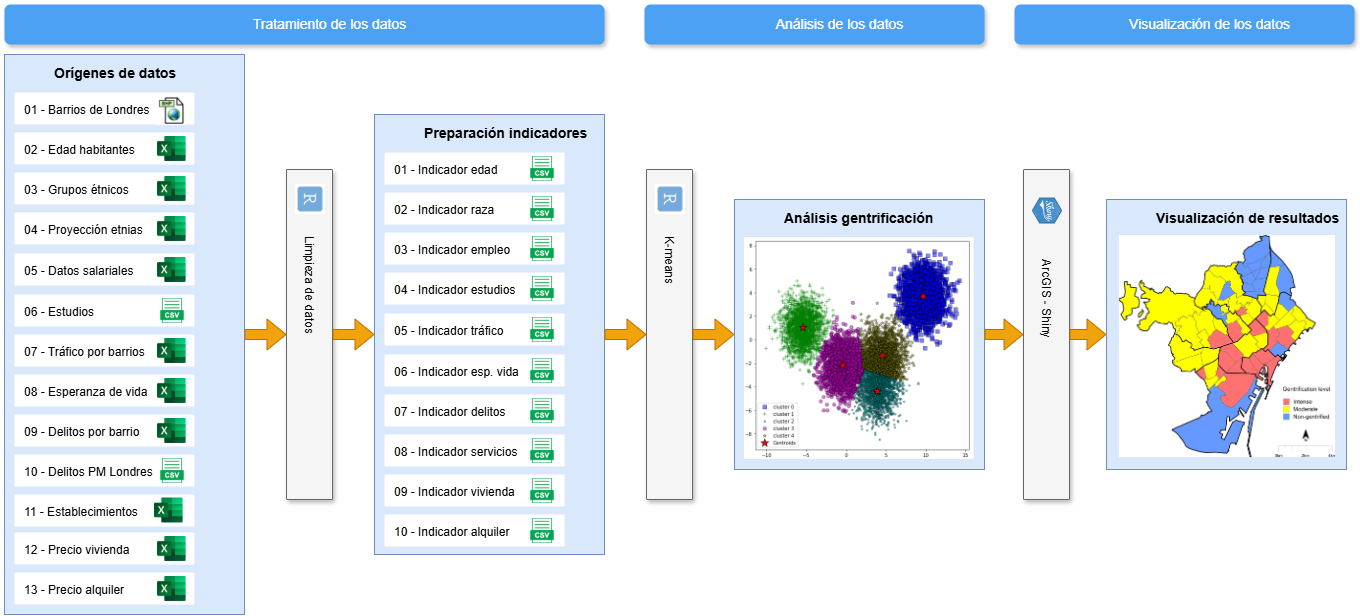
\includegraphics[width=1\linewidth]{TFM_Plantilla 2//jgoncasTFM0125memoria//figs//M3/esquema_tratamiento_datos_v2.png}
    \caption{Etapas del procesamiento de los datos}
    \label{fig:fig_procesamiento_datos}
\end{figure}

A continuación, detallamos el proceso seguido con cada uno de los indicadores en la primera fase de limpieza y procesamiento de los datos.

\subsection{Indicador 01: Edad media de la población}

Este primer indicador corresponde con el registro número 2 de la tabla \ref{tab:tab_fuentes} y nace de los datos estimados en base a los resultados de los diferentes censos de la ciudad de Londres.

\subsubsection{Formato de entrada}

El fichero del origen de datos se trata de un Excel con un registro para cada barrio de Londres entre los años 1999 y 2020. Aparte, hay registros por áreas que agrupan los datos según la ubicación geográfica de los barrios en base a su pertenencia al anillo exterior de la ciudad (Outer London) o a la parte interior (Inner London). También se dispone de datos para Gales, Escocia y Reino Unido. Estas agrupaciones son habituales encontrarlas en el resto de orígenes de datos utilizados dentro de este trabajo.

Para cada uno de los registros correspondientes a un barrio y a un año, se dispone de datos de la cantidad de personas según su edad, desde los 0 años hasta los 89 y un último grupo para personas con 90 o más años. Esta información está dividida por género (masculino y femenino). 

Existe una excepción para este esquema en los años 1999 y 2000, donde los grupos de edad van desde los 0 hasta los 84 años, registrando a todas las personas de 85 y más años dentro de la misma celda. Como los datos con los que se trabaja en este estudio parten del año 2001, los registros para los años anteriores serán eliminados de la muestra, no afectando la circunstancia que mencionamos en el resto del trabajo de limpieza de los datos.

\subsubsection{Pasos del proceso de limpieza}

\begin{enumerate}
    \item \textbf{Lectura del fichero}: Como se puede apreciar de forma parcial en la figura \ref{fig:fig_fichero_ind_01}, se compone la lista de columnas a leer en el Excel de entrada indicando el nombre que utilizaremos. El dataframe resultado tendrá las columnas "Code", "Year", "Borough", una lista de 91 columnas con formato "M\_x", donde la x corresponde con la edad de las personas de género masculino, la columna "No\_Males" que se encuentra intercalada en el origen de datos entre la información del género masculino y el género femenino y, para finalizar, una lista de 91 columnas con el formato "F\_x", para la edad de las personas de género femenino.
    \item \textbf{Eliminación de columnas}: Se elimina la columna "No\_Males" pues no contiene información relevante
    \item \textbf{Filtra barrios de Londres}: Elimina aquellos registros que no se corresponden con barrios de Londres o al global de la ciudad
    \item \textbf{Eliminación datos antiguos}: Se eliminan aquellos registros anteriores al año 2001
    \item \textbf{Cálculo de la edad media}: Se obtiene el valor de la edad media por barrio y año independientemente del género
    \item \textbf{Eliminación datos por edad}: Una vez calculada la edad media, se eliminan los datos desagregados del dataframe
    \item \textbf{Estimación de datos}: Utilizando el modelo ARIMA, se estiman la edad media por barrio y año desde 2021 hasta 2031 tomando como base los valores de la serie temporal que se genera con los datos desde el año 2000 hasta el año 2020
\end{enumerate}

\begin{figure}
    \centering
    \includegraphics[width=0.75\linewidth]{TFM_Plantilla 2//jgoncasTFM0125memoria//figs//M3/m3_fichero_ind_01.png}
    \caption{Formato del fichero de entrada para el indicador de edad}
    \label{fig:fig_fichero_ind_01}
\end{figure}

\subsection{Indicador 02: Población de raza blanca}

Este indicador tiene dos orígenes de datos, debido a que en el London Datastore hay información de los grupos étnicos por barrio desde 2001 hasta 2009. Sin embargo, para datos más recientes se ha obtenido la información del Urban Big Data Centre. Los orígenes corresponden con los registros 3 y 4 del cuadro \ref{tab:tab_fuentes}.

\subsubsection{Formato de entrada}

Aunque en ambos casos el formato de los ficheros de entrada varía la información que contienen es similar y se corresponde con la cantidad de habitantes por barrio que pertenecen a un grupo étnico concreto. En el caso de los datos disponibles a partir de 2011, esta información viene agrupada por edad. En ambos casos tenemos una serie de grupos étnicos que clasificaremos en dos grupos: "\textit{White}" o "\textit{BAME}" que es el término utilizado para englobar a personas de raza negra (B), asiática (A) y minorías étnicas (ME). En el conjunto de raza blanca están incluidos británicos e irlandeses de raza blanca y otros de esta misma raza. La figura \ref{fig:fig_clasificacion_razas} muestra esta clasificación.

\begin{figure}
    \centering
    \includegraphics[width=1\linewidth]{TFM_Plantilla 2//jgoncasTFM0125memoria//figs//M3/m3_clasificacion_razas.png}
    \caption{Clasificación de grupos raciales}
    \label{fig:fig_clasificacion_razas}
\end{figure}

En el caso de los datos desde 2001 hasta 2009, el fichero contiene una pestaña por año. Cada fila de la hoja corresponde con un barrio, mientras que las columnas corresponden al conteo de cada grupo étnico para ese barrio dividido entre 1000 en tres grupos, el total por género y un grupo por género (femenino y masculino).

En cambio, los datos entre 2011 y 2050 se encuentran todos en una misma pestaña, desglosados por barrio, edad y grupo étnico. Cada columna pues, consta de los datos para cada uno de los años indicados. Al tratarse de datos estimados, la proyección de los mismos se ha realizado de forma consistente con la tendencia central de los datos respecto al año 2016.

\subsubsection{Pasos del proceso de limpieza}

La secuencia de pasos seguida para el proceso de limpieza de los datos de este indicador ha sido la siguiente:

\begin{enumerate}
    \item \textbf{Eliminación de columnas por género}: Eliminación de los datos de género femenino y masculino leídos en el primer fichero.
    \item \textbf{Normalización de nombre}: Se actualiza el registro para los datos globales de Londres para sustituir el nombre "LONDON" por "London"
    \item \textbf{Filtra barrios de Londres}: Elimina aquellos registros que no se corresponden con barrios de Londres o al global de la ciudad
    \item \textbf{Actualiza los valores}: Como en el primero de los ficheros los datos venían divididos entre 1000, se realiza la operación inversa para usar la misma medida cuando se unifique con los datos del segundo fichero
    \item \textbf{Estimación de datos año 2010}: Al existir un hueco de un año entre los datos de los dos ficheros del origen de datos de este indicador, usamos el modelo ARIMA para predecir el valor de cada grupo étnico en cada barrio para el año 2010
\end{enumerate}

\subsection{Indicador 03: Salario medio semanal}

\subsection{Indicador 04: Porcentaje de población con estudios superiores}

\subsection{Indicador 05: Cantidad de tráfico de vehículos}

\subsection{Indicador 06: Esperanza de vida}

\subsection{Indicador 07: Cantidad de delitos a la semana}

\subsection{Indicador 08: Cantidad de servicios en la zona (restaurantes y tiendas)}

\subsection{Indicador 09: Precio medio de la vivienda}

\subsection{Indicador 10: Precio medio del alquiler social}

\chapter{Resultados y conclusiones}

% NOTAS
1) Indicador 1: Edad

1.1) Imputación de valores nulos
En los años 1999 y 2000 los datos se obtenían desde 0 hasta 84 años y el resto se incluían en 85+, a partir de 2001 este recuento varía entre 0 y 89 y un grupo 90+. Lo que hacemos con los valores NA esos dos años es dividir el valor de 85+ en los grupos de edad 85, 86, 87, 88, 89 y 90

\begin{figure}
    \centering
    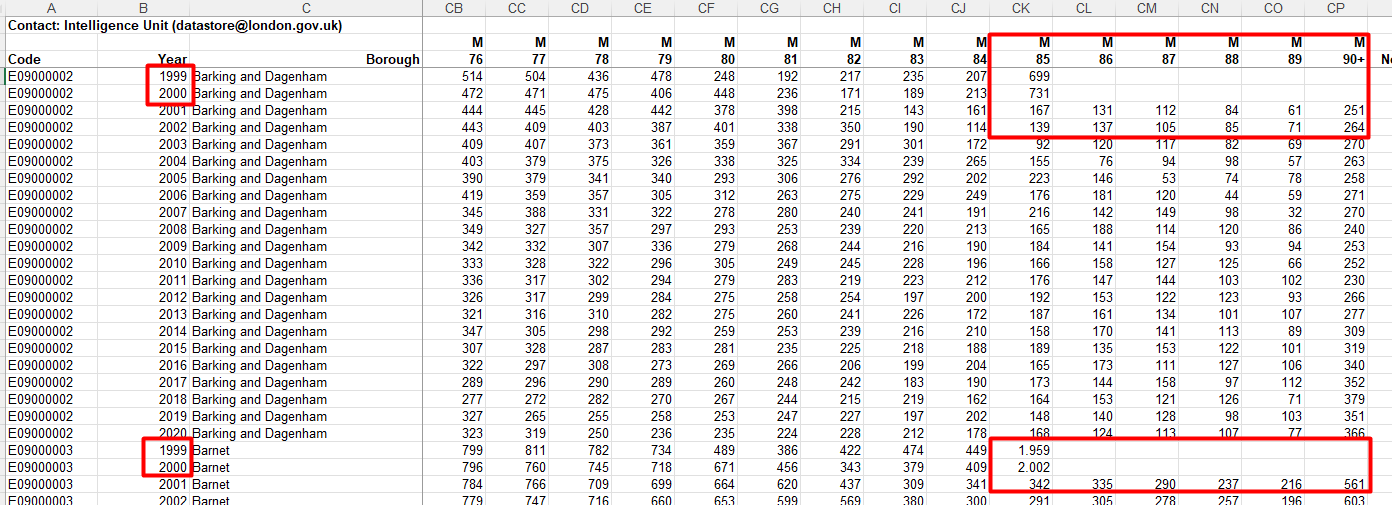
\includegraphics[width=0.75\linewidth]{TFM_Plantilla 2//jgoncasTFM0125memoria//images//M3/m3_imputaciones_datos_edad.png}
    \caption{Enter Caption}
    \label{fig:enter-label}
\end{figure}

4) Indicador 4: Estudios

Se imputa el valor del 80\% donde no se tiene porcentaje calculado, para el resto se asigna el valor correspondiente

\begin{figure}
    \centering
    \includegraphics[width=0.75\linewidth]{TFM_Plantilla 2//jgoncasTFM0125memoria//images//M3/m3_imputacion_estudios.png}
    \caption{Enter Caption}
    \label{fig:enter-label}
\end{figure}

% FUENTE DATOS
% 0) Barrios de Londres
%   - https://data.london.gov.uk/dataset/london_boroughs --> Paquete GPKG
%   - https://data.london.gov.uk/dataset/statistical-gis-boundary-files-london --> Shapefiles
% 1) Indicadores demográficos
%   - https://data.london.gov.uk/dataset/ethnic-groups-borough --> ethnic-groups-by-borough.xls
%   - https://data.london.gov.uk/dataset/ons-mid-year-population-estimates-custom-age-tables --> ons-mye-custom-age-tool-2020.xlsx
% 2) Indicadores económicos
%   - https://data.london.gov.uk/dataset/earnings-place-residence-borough --> 
% 3) Indicadores educativos
%   - https://data.london.gov.uk/dataset/qualifications-working-age-population-nvq-borough --> Qualifications-of-working-age-NVQ.csv
% 4) Indicadores medioambientales
%   - https://data.london.gov.uk/dataset/traffic-flows-borough --> traffic-flow-borough.xls
% 5) Indicadores sanitarios
%   - https://data.london.gov.uk/dataset/life-expectancy-birth-and-age-65-borough --> life-expectancy-birth-over65-borough.xls
% 6) Indicadores de seguridad
%   - https://data.london.gov.uk/dataset/recorded_crime_summary --> MPS Borough Level Crime (Historical).csv
% 7) Indicadores sobre servicios
%   - https://data.london.gov.uk/dataset/local-units-broad-industry-group-borough --> local-units-by-broad-industry-group.xls
%   - Plan B: https://data.london.gov.uk/dataset/pubs-clubs-restaurants-takeaways-borough --> take-away-borough.xls, pubs-borough-msoa.xls, licensed-restaurants-cafes-borough.xls
% 8) Indicadores sobre vivienda
%   - https://data.london.gov.uk/dataset/average-house-prices --> land-registry-house-prices-borough.xls
%   - https://data.london.gov.uk/dataset/registered-social-landlords-average-rents --> social-landlord-rents-borough.xls

\chapter{Conclusiones y trabajo futuro}

\chapter{Glosario}

\begin{itemize}
    \item \textbf{BME}: Acrónimo que refiere a grupos de personas de raza negra y otros grupos étnicos minoritarios
    \item \textbf{Cronograma}: Herramienta de planificación de proyectos que representa de manera visual el conjunto de actividades o tareas a realizar.
    \item \textbf{Data Store}: Repositorio o almacén de datos.
    \item \textbf{Datos geoespaciales}: Datos que incluyen alguna componente geográfica, como la latitud y la longitud que permite ubicarlos dentro de la superficie terrestre.
    \item \textbf{Diagrama de Gantt}: Herramienta gráfica utilizada en la gestión de proyectos para representar visualmente el cronograma de actividades o tareas.
    \item \textbf{Gentrificación}: Proceso de transformación urbana en el que debido al incremento de valor por nuevas inversiones atrae la llegada de nuevos residentes con mayor poder adquisitivo y que suele llevar al desplazamiento de los habitantes originales de clases trabajadoras a otras zonas de la ciudad.
    \item \textbf{Gentrificación verde}: Procesos de gentrificación urbana basados en la creación o restauración de amenidades ambientales.
    \item \textbf{IDE}: Acrónimo de Integrated Development Environment o entorno de desarrollo integrado, que es un software que incluye herramientas de desarrollo de software, como un editor, un depurador y herramientas de compilación e integración.
    \item \textbf{LTN}: Acrónimo de Low Traffic Neighborhood, que es una iniciativa diseñada para reducir el tráfico, limitando el acceso de vehículos en ciertas zonas creando entornos más seguros y sostenibles.
    \item \textbf{Scrum}: Marco de trabajo ágil utilizado en la gestión de proyectos para facilitar la colaboración en equipos de desarrollo. Se basa en ciclos cortos y repetitivos llamados sprints donde el objetivo es completar tareas específicas para entregar incrementos funcionales del producto.
    \item \textbf{Segregación}: Separación o aislamiento de un grupo de personas por razones sociales, étnicas, religiosas o de otra índole con la consecuencia de limitar su acceso a recursos u oportunidades. 
    \item \textbf{Sprint}: En el contexto de la gestión ágil de proyectos y, en particular, de la metodología Scrum, un sprint es un ciclo corto de trabajo durante el cual el equipo de desarrollo trabaja en completar un conjunto definido de tareas o historias de usuario.
    \item \textbf{TFM}: Acrónimo de Trabajo Final de Máster
    \item \textbf{UBDC}: Acrónimo de Urban Big Data Centre, entidad dedicada al análisis de datos urbanos a gran escala.
\end{itemize}

% bibliografía
\addcontentsline{toc}{chapter}{Bibliografía}
%\bibliographystyle{unsrt}
\bibliographystyle{plain}
\bibliography{referencias}

%\chapter{Anexos}

\end{document}
